\documentclass[twoside]{book}

% Packages required by doxygen
\usepackage{fixltx2e}
\usepackage{calc}
\usepackage{doxygen}
\usepackage[export]{adjustbox} % also loads graphicx
\usepackage{graphicx}
\usepackage[utf8]{inputenc}
\usepackage{makeidx}
\usepackage{multicol}
\usepackage{multirow}
\PassOptionsToPackage{warn}{textcomp}
\usepackage{textcomp}
\usepackage[nointegrals]{wasysym}
\usepackage[table]{xcolor}

% Font selection
\usepackage[T1]{fontenc}
\usepackage[scaled=.90]{helvet}
\usepackage{courier}
\usepackage{amssymb}
\usepackage{sectsty}
\renewcommand{\familydefault}{\sfdefault}
\allsectionsfont{%
  \fontseries{bc}\selectfont%
  \color{darkgray}%
}
\renewcommand{\DoxyLabelFont}{%
  \fontseries{bc}\selectfont%
  \color{darkgray}%
}
\newcommand{\+}{\discretionary{\mbox{\scriptsize$\hookleftarrow$}}{}{}}

% Page & text layout
\usepackage{geometry}
\geometry{%
  a4paper,%
  top=2.5cm,%
  bottom=2.5cm,%
  left=2.5cm,%
  right=2.5cm%
}
\tolerance=750
\hfuzz=15pt
\hbadness=750
\setlength{\emergencystretch}{15pt}
\setlength{\parindent}{0cm}
\setlength{\parskip}{3ex plus 2ex minus 2ex}
\makeatletter
\renewcommand{\paragraph}{%
  \@startsection{paragraph}{4}{0ex}{-1.0ex}{1.0ex}{%
    \normalfont\normalsize\bfseries\SS@parafont%
  }%
}
\renewcommand{\subparagraph}{%
  \@startsection{subparagraph}{5}{0ex}{-1.0ex}{1.0ex}{%
    \normalfont\normalsize\bfseries\SS@subparafont%
  }%
}
\makeatother

% Headers & footers
\usepackage{fancyhdr}
\pagestyle{fancyplain}
\fancyhead[LE]{\fancyplain{}{\bfseries\thepage}}
\fancyhead[CE]{\fancyplain{}{}}
\fancyhead[RE]{\fancyplain{}{\bfseries\leftmark}}
\fancyhead[LO]{\fancyplain{}{\bfseries\rightmark}}
\fancyhead[CO]{\fancyplain{}{}}
\fancyhead[RO]{\fancyplain{}{\bfseries\thepage}}
\fancyfoot[LE]{\fancyplain{}{}}
\fancyfoot[CE]{\fancyplain{}{}}
\fancyfoot[RE]{\fancyplain{}{\bfseries\scriptsize Generated by Doxygen }}
\fancyfoot[LO]{\fancyplain{}{\bfseries\scriptsize Generated by Doxygen }}
\fancyfoot[CO]{\fancyplain{}{}}
\fancyfoot[RO]{\fancyplain{}{}}
\renewcommand{\footrulewidth}{0.4pt}
\renewcommand{\chaptermark}[1]{%
  \markboth{#1}{}%
}
\renewcommand{\sectionmark}[1]{%
  \markright{\thesection\ #1}%
}

% Indices & bibliography
\usepackage{natbib}
\usepackage[titles]{tocloft}
\setcounter{tocdepth}{3}
\setcounter{secnumdepth}{5}
\makeindex

% Hyperlinks (required, but should be loaded last)
\usepackage{ifpdf}
\ifpdf
  \usepackage[pdftex,pagebackref=true]{hyperref}
\else
  \usepackage[ps2pdf,pagebackref=true]{hyperref}
\fi
\hypersetup{%
  colorlinks=true,%
  linkcolor=blue,%
  citecolor=blue,%
  unicode%
}

% Custom commands
\newcommand{\clearemptydoublepage}{%
  \newpage{\pagestyle{empty}\cleardoublepage}%
}

\usepackage{caption}
\captionsetup{labelsep=space,justification=centering,font={bf},singlelinecheck=off,skip=4pt,position=top}

%===== C O N T E N T S =====

\begin{document}

% Titlepage & ToC
\hypersetup{pageanchor=false,
             bookmarksnumbered=true,
             pdfencoding=unicode
            }
\pagenumbering{alph}
\begin{titlepage}
\vspace*{7cm}
\begin{center}%
{\Large Minecraftchest1 }\\
\vspace*{1cm}
{\large Generated by Doxygen 1.8.13}\\
\end{center}
\end{titlepage}
\clearemptydoublepage
\pagenumbering{roman}
\tableofcontents
\clearemptydoublepage
\pagenumbering{arabic}
\hypersetup{pageanchor=true}

%--- Begin generated contents ---
\chapter{Minecraftchest1-\/utils}
\label{autotoc_md0}
\Hypertarget{autotoc_md0}
All methods are located under the {\ttfamily Utils} class in the {\ttfamily \hyperlink{namespace_minecraftchest1}{Minecraftchest1}} namespace.

Documentation is automaticly generated,and can be found at \href{https://minecraftchest1.github.io/nuget-packages/class_minecraftchest1_1_1_utils.html}{\tt https\+://minecraftchest1.\+github.\+io/nuget-\/packages/class\+\_\+minecraftchest1\+\_\+1\+\_\+1\+\_\+utils.\+html} 
\chapter{Namespace Index}
\section{Namespace List}
Here is a list of all documented namespaces with brief descriptions\+:\begin{DoxyCompactList}
\item\contentsline{section}{\hyperlink{namespace_minecraftchest1}{Minecraftchest1} }{\pageref{namespace_minecraftchest1}}{}
\end{DoxyCompactList}

\chapter{Hierarchical Index}
\doxysection{Class Hierarchy}
This inheritance list is sorted roughly, but not completely, alphabetically\+:\begin{DoxyCompactList}
\item Exception\begin{DoxyCompactList}
\item \contentsline{section}{Minecraftchest1.\+Utils.\+Input\+Error\+Exception}{\pageref{class_minecraftchest1_1_1_utils_1_1_input_error_exception}}{}
\end{DoxyCompactList}
\item \contentsline{section}{Minecraftchest1.\+Utils}{\pageref{class_minecraftchest1_1_1_utils}}{}
\end{DoxyCompactList}

\chapter{Class Index}
\doxysection{Class List}
Here are the classes, structs, unions and interfaces with brief descriptions\+:\begin{DoxyCompactList}
\item\contentsline{section}{\mbox{\hyperlink{class_minecraftchest1_1_1_utils_1_1_input_error_exception}{Minecraftchest1.\+Utils.\+Input\+Error\+Exception}} }{\pageref{class_minecraftchest1_1_1_utils_1_1_input_error_exception}}{}
\item\contentsline{section}{\mbox{\hyperlink{class_minecraftchest1_1_1_utils}{Minecraftchest1.\+Utils}} }{\pageref{class_minecraftchest1_1_1_utils}}{}
\end{DoxyCompactList}

\chapter{Namespace Documentation}
\hypertarget{namespace_minecraftchest1}{}\doxysection{Minecraftchest1 Namespace Reference}
\label{namespace_minecraftchest1}\index{Minecraftchest1@{Minecraftchest1}}
\doxysubsection*{Classes}
\begin{DoxyCompactItemize}
\item 
class \mbox{\hyperlink{class_minecraftchest1_1_1_utils}{Utils}}
\end{DoxyCompactItemize}

\chapter{Class Documentation}
\hypertarget{class_minecraftchest1_1_1_utils_1_1_input_error_exception}{}\doxysection{Minecraftchest1.\+Utils.\+Input\+Error\+Exception Class Reference}
\label{class_minecraftchest1_1_1_utils_1_1_input_error_exception}\index{Minecraftchest1.Utils.InputErrorException@{Minecraftchest1.Utils.InputErrorException}}
Inheritance diagram for Minecraftchest1.\+Utils.\+Input\+Error\+Exception\+:\begin{figure}[H]
\begin{center}
\leavevmode
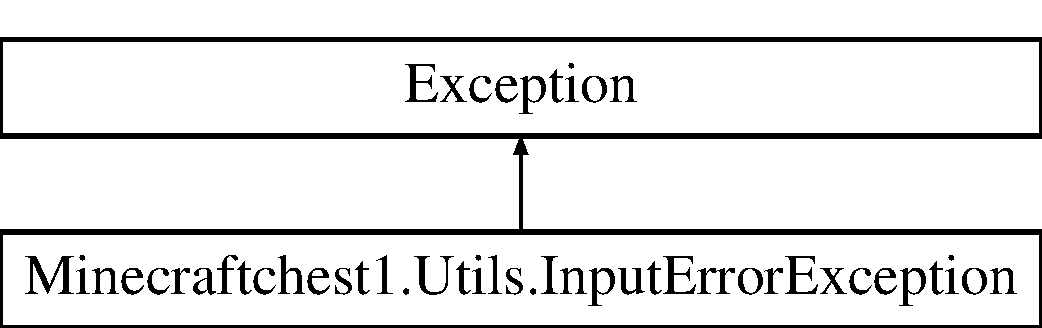
\includegraphics[height=2.000000cm]{class_minecraftchest1_1_1_utils_1_1_input_error_exception}
\end{center}
\end{figure}
\doxysubsection*{Public Member Functions}
\begin{DoxyCompactItemize}
\item 
\mbox{\hyperlink{class_minecraftchest1_1_1_utils_1_1_input_error_exception_a1bda68cd00bf63e46e593edaf8a5e57b}{Input\+Error\+Exception}} (string message)
\item 
\mbox{\hyperlink{class_minecraftchest1_1_1_utils_1_1_input_error_exception_a38a7a2f9f54188ccd25a524886dd77d4}{Input\+Error\+Exception}} (string message, Exception inner)
\end{DoxyCompactItemize}
\doxysubsection*{Public Attributes}
\begin{DoxyCompactItemize}
\item 
string \mbox{\hyperlink{class_minecraftchest1_1_1_utils_1_1_input_error_exception_a9da985457dab9915b3cd79cb13cc6683}{Input}}
\end{DoxyCompactItemize}
\doxysubsection*{Protected Member Functions}
\begin{DoxyCompactItemize}
\item 
\mbox{\hyperlink{class_minecraftchest1_1_1_utils_1_1_input_error_exception_aa0a4f5a18c8d9973bbb9fa003278e2a1}{Input\+Error\+Exception}} (System.\+Runtime.\+Serialization.\+Serialization\+Info info, System.\+Runtime.\+Serialization.\+Streaming\+Context context)
\end{DoxyCompactItemize}


\doxysubsection{Detailed Description}


Definition at line \mbox{\hyperlink{_exceptions_8cs_source_l00008}{8}} of file \mbox{\hyperlink{_exceptions_8cs_source}{Exceptions.\+cs}}.



\doxysubsection{Constructor \& Destructor Documentation}
\mbox{\Hypertarget{class_minecraftchest1_1_1_utils_1_1_input_error_exception_a6e4779b6fe0b6101969ff84af4fcdf1a}\label{class_minecraftchest1_1_1_utils_1_1_input_error_exception_a6e4779b6fe0b6101969ff84af4fcdf1a}} 
\index{Minecraftchest1.Utils.InputErrorException@{Minecraftchest1.Utils.InputErrorException}!InputErrorException@{InputErrorException}}
\index{InputErrorException@{InputErrorException}!Minecraftchest1.Utils.InputErrorException@{Minecraftchest1.Utils.InputErrorException}}
\doxysubsubsection{\texorpdfstring{InputErrorException()}{InputErrorException()}\hspace{0.1cm}{\footnotesize\ttfamily [1/4]}}
{\footnotesize\ttfamily Minecraftchest1.\+Utils.\+Input\+Error\+Exception.\+Input\+Error\+Exception (\begin{DoxyParamCaption}{ }\end{DoxyParamCaption})\hspace{0.3cm}{\ttfamily [inline]}}



Definition at line \mbox{\hyperlink{_exceptions_8cs_source_l00010}{10}} of file \mbox{\hyperlink{_exceptions_8cs_source}{Exceptions.\+cs}}.

\mbox{\Hypertarget{class_minecraftchest1_1_1_utils_1_1_input_error_exception_a1bda68cd00bf63e46e593edaf8a5e57b}\label{class_minecraftchest1_1_1_utils_1_1_input_error_exception_a1bda68cd00bf63e46e593edaf8a5e57b}} 
\index{Minecraftchest1.Utils.InputErrorException@{Minecraftchest1.Utils.InputErrorException}!InputErrorException@{InputErrorException}}
\index{InputErrorException@{InputErrorException}!Minecraftchest1.Utils.InputErrorException@{Minecraftchest1.Utils.InputErrorException}}
\doxysubsubsection{\texorpdfstring{InputErrorException()}{InputErrorException()}\hspace{0.1cm}{\footnotesize\ttfamily [2/4]}}
{\footnotesize\ttfamily Minecraftchest1.\+Utils.\+Input\+Error\+Exception.\+Input\+Error\+Exception (\begin{DoxyParamCaption}\item[{string}]{message }\end{DoxyParamCaption})\hspace{0.3cm}{\ttfamily [inline]}}



Definition at line \mbox{\hyperlink{_exceptions_8cs_source_l00011}{11}} of file \mbox{\hyperlink{_exceptions_8cs_source}{Exceptions.\+cs}}.

\mbox{\Hypertarget{class_minecraftchest1_1_1_utils_1_1_input_error_exception_a38a7a2f9f54188ccd25a524886dd77d4}\label{class_minecraftchest1_1_1_utils_1_1_input_error_exception_a38a7a2f9f54188ccd25a524886dd77d4}} 
\index{Minecraftchest1.Utils.InputErrorException@{Minecraftchest1.Utils.InputErrorException}!InputErrorException@{InputErrorException}}
\index{InputErrorException@{InputErrorException}!Minecraftchest1.Utils.InputErrorException@{Minecraftchest1.Utils.InputErrorException}}
\doxysubsubsection{\texorpdfstring{InputErrorException()}{InputErrorException()}\hspace{0.1cm}{\footnotesize\ttfamily [3/4]}}
{\footnotesize\ttfamily Minecraftchest1.\+Utils.\+Input\+Error\+Exception.\+Input\+Error\+Exception (\begin{DoxyParamCaption}\item[{string}]{message,  }\item[{Exception}]{inner }\end{DoxyParamCaption})\hspace{0.3cm}{\ttfamily [inline]}}



Definition at line \mbox{\hyperlink{_exceptions_8cs_source_l00012}{12}} of file \mbox{\hyperlink{_exceptions_8cs_source}{Exceptions.\+cs}}.

\mbox{\Hypertarget{class_minecraftchest1_1_1_utils_1_1_input_error_exception_aa0a4f5a18c8d9973bbb9fa003278e2a1}\label{class_minecraftchest1_1_1_utils_1_1_input_error_exception_aa0a4f5a18c8d9973bbb9fa003278e2a1}} 
\index{Minecraftchest1.Utils.InputErrorException@{Minecraftchest1.Utils.InputErrorException}!InputErrorException@{InputErrorException}}
\index{InputErrorException@{InputErrorException}!Minecraftchest1.Utils.InputErrorException@{Minecraftchest1.Utils.InputErrorException}}
\doxysubsubsection{\texorpdfstring{InputErrorException()}{InputErrorException()}\hspace{0.1cm}{\footnotesize\ttfamily [4/4]}}
{\footnotesize\ttfamily Minecraftchest1.\+Utils.\+Input\+Error\+Exception.\+Input\+Error\+Exception (\begin{DoxyParamCaption}\item[{System.\+Runtime.\+Serialization.\+Serialization\+Info}]{info,  }\item[{System.\+Runtime.\+Serialization.\+Streaming\+Context}]{context }\end{DoxyParamCaption})\hspace{0.3cm}{\ttfamily [inline]}, {\ttfamily [protected]}}



Definition at line \mbox{\hyperlink{_exceptions_8cs_source_l00013}{13}} of file \mbox{\hyperlink{_exceptions_8cs_source}{Exceptions.\+cs}}.



\doxysubsection{Member Data Documentation}
\mbox{\Hypertarget{class_minecraftchest1_1_1_utils_1_1_input_error_exception_a9da985457dab9915b3cd79cb13cc6683}\label{class_minecraftchest1_1_1_utils_1_1_input_error_exception_a9da985457dab9915b3cd79cb13cc6683}} 
\index{Minecraftchest1.Utils.InputErrorException@{Minecraftchest1.Utils.InputErrorException}!Input@{Input}}
\index{Input@{Input}!Minecraftchest1.Utils.InputErrorException@{Minecraftchest1.Utils.InputErrorException}}
\doxysubsubsection{\texorpdfstring{Input}{Input}}
{\footnotesize\ttfamily string Minecraftchest1.\+Utils.\+Input\+Error\+Exception.\+Input}



Definition at line \mbox{\hyperlink{_exceptions_8cs_source_l00017}{17}} of file \mbox{\hyperlink{_exceptions_8cs_source}{Exceptions.\+cs}}.



The documentation for this class was generated from the following file\+:\begin{DoxyCompactItemize}
\item 
utils/Exceptions.\+cs\end{DoxyCompactItemize}

\hypertarget{class_minecraftchest1_1_1_utils}{}\doxysection{Minecraftchest1.\+Utils Class Reference}
\label{class_minecraftchest1_1_1_utils}\index{Minecraftchest1.Utils@{Minecraftchest1.Utils}}
\doxysubsection*{Classes}
\begin{DoxyCompactItemize}
\item 
class \mbox{\hyperlink{class_minecraftchest1_1_1_utils_1_1_input_error_exception}{Input\+Error\+Exception}}
\end{DoxyCompactItemize}
\doxysubsection*{Static Public Member Functions}
\begin{DoxyCompactItemize}
\item 
static void \mbox{\hyperlink{class_minecraftchest1_1_1_utils_a93d87d31f16115eb3ef2da07ef774530}{Pause}} (string Message=\char`\"{}Press any key to continue...\char`\"{}, bool Seperator=false)
\item 
static string \mbox{\hyperlink{class_minecraftchest1_1_1_utils_acc8f15ceee7fa0c1c521cdb582bc3910}{Input}} (string prompt)
\item 
static double \mbox{\hyperlink{class_minecraftchest1_1_1_utils_a0f88327089e8a17005bc3c7981487c32}{Input\+Double}} (string prompt)
\item 
static byte \mbox{\hyperlink{class_minecraftchest1_1_1_utils_abd4c72e46dc83dc796229b1bfa187d80}{Input\+Byte}} (string prompt)
\item 
\mbox{\Hypertarget{class_minecraftchest1_1_1_utils_a4ea88face18276bc3c7e70a212f63b4a}\label{class_minecraftchest1_1_1_utils_a4ea88face18276bc3c7e70a212f63b4a}} 
static string\mbox{[}$\,$\mbox{]} {\bfseries String\+To\+Array} (string \mbox{\hyperlink{class_minecraftchest1_1_1_utils_acc8f15ceee7fa0c1c521cdb582bc3910}{Input}}, char\mbox{[}$\,$\mbox{]} Seperators)
\item 
\mbox{\Hypertarget{class_minecraftchest1_1_1_utils_adc4fd4490e43598e7c07908dcc814458}\label{class_minecraftchest1_1_1_utils_adc4fd4490e43598e7c07908dcc814458}} 
static string {\bfseries Array\+To\+String} (string\mbox{[}$\,$\mbox{]} \mbox{\hyperlink{class_minecraftchest1_1_1_utils_acc8f15ceee7fa0c1c521cdb582bc3910}{Input}}, char Seperator)
\item 
static void \mbox{\hyperlink{class_minecraftchest1_1_1_utils_a009121f4c8753027691de96462294d92}{Exit}} (Int32 exit\+Code=0)
\item 
static byte \mbox{\hyperlink{class_minecraftchest1_1_1_utils_a035e281ebdbe7cc5fc010c187beb85cf}{Menu}} (Dictionary$<$ byte, string $>$ menu)
\end{DoxyCompactItemize}


\doxysubsection{Member Function Documentation}
\mbox{\Hypertarget{class_minecraftchest1_1_1_utils_a009121f4c8753027691de96462294d92}\label{class_minecraftchest1_1_1_utils_a009121f4c8753027691de96462294d92}} 
\index{Minecraftchest1.Utils@{Minecraftchest1.Utils}!Exit@{Exit}}
\index{Exit@{Exit}!Minecraftchest1.Utils@{Minecraftchest1.Utils}}
\doxysubsubsection{\texorpdfstring{Exit()}{Exit()}}
{\footnotesize\ttfamily static void Minecraftchest1.\+Utils.\+Exit (\begin{DoxyParamCaption}\item[{Int32}]{exit\+Code = {\ttfamily 0} }\end{DoxyParamCaption})\hspace{0.3cm}{\ttfamily [inline]}, {\ttfamily [static]}}

Exits the application. /summary$>$ param name=\char`\"{}exit\+Code\char`\"{}$>$ Error code to provide when exiting. Defaults to 0 (successful). /param$>$\mbox{\Hypertarget{class_minecraftchest1_1_1_utils_acc8f15ceee7fa0c1c521cdb582bc3910}\label{class_minecraftchest1_1_1_utils_acc8f15ceee7fa0c1c521cdb582bc3910}} 
\index{Minecraftchest1.Utils@{Minecraftchest1.Utils}!Input@{Input}}
\index{Input@{Input}!Minecraftchest1.Utils@{Minecraftchest1.Utils}}
\doxysubsubsection{\texorpdfstring{Input()}{Input()}}
{\footnotesize\ttfamily static string Minecraftchest1.\+Utils.\+Input (\begin{DoxyParamCaption}\item[{string}]{prompt }\end{DoxyParamCaption})\hspace{0.3cm}{\ttfamily [inline]}, {\ttfamily [static]}}

Asks for user input. 


\begin{DoxyParams}{Parameters}
{\em prompt} & The message to show when asking for input. Dispalyed on the same line of the input prompt. \\
\hline
\end{DoxyParams}
\begin{DoxyReturn}{Returns}
Returns the input from the user. 
\end{DoxyReturn}
\mbox{\Hypertarget{class_minecraftchest1_1_1_utils_abd4c72e46dc83dc796229b1bfa187d80}\label{class_minecraftchest1_1_1_utils_abd4c72e46dc83dc796229b1bfa187d80}} 
\index{Minecraftchest1.Utils@{Minecraftchest1.Utils}!InputByte@{InputByte}}
\index{InputByte@{InputByte}!Minecraftchest1.Utils@{Minecraftchest1.Utils}}
\doxysubsubsection{\texorpdfstring{InputByte()}{InputByte()}}
{\footnotesize\ttfamily static byte Minecraftchest1.\+Utils.\+Input\+Byte (\begin{DoxyParamCaption}\item[{string}]{prompt }\end{DoxyParamCaption})\hspace{0.3cm}{\ttfamily [inline]}, {\ttfamily [static]}}

Asks for user input. Returns a byte. 

Returns 0 when no user input is provided. 


\begin{DoxyParams}{Parameters}
{\em prompt} & The message to show when asking for input. Dispalyed on the same line of the input prompt. \\
\hline
\end{DoxyParams}
\begin{DoxyReturn}{Returns}
Returns the input from the user. 
\end{DoxyReturn}
\mbox{\Hypertarget{class_minecraftchest1_1_1_utils_a0f88327089e8a17005bc3c7981487c32}\label{class_minecraftchest1_1_1_utils_a0f88327089e8a17005bc3c7981487c32}} 
\index{Minecraftchest1.Utils@{Minecraftchest1.Utils}!InputDouble@{InputDouble}}
\index{InputDouble@{InputDouble}!Minecraftchest1.Utils@{Minecraftchest1.Utils}}
\doxysubsubsection{\texorpdfstring{InputDouble()}{InputDouble()}}
{\footnotesize\ttfamily static double Minecraftchest1.\+Utils.\+Input\+Double (\begin{DoxyParamCaption}\item[{string}]{prompt }\end{DoxyParamCaption})\hspace{0.3cm}{\ttfamily [inline]}, {\ttfamily [static]}}

Asks for user input. Returns a double. 

Returns 0 when no user input is provided. 


\begin{DoxyParams}{Parameters}
{\em prompt} & The message to show when asking for input. Dispalyed on the same line of the input prompt. \\
\hline
\end{DoxyParams}
\begin{DoxyReturn}{Returns}
Returns the input from the user. 
\end{DoxyReturn}
\mbox{\Hypertarget{class_minecraftchest1_1_1_utils_a035e281ebdbe7cc5fc010c187beb85cf}\label{class_minecraftchest1_1_1_utils_a035e281ebdbe7cc5fc010c187beb85cf}} 
\index{Minecraftchest1.Utils@{Minecraftchest1.Utils}!Menu@{Menu}}
\index{Menu@{Menu}!Minecraftchest1.Utils@{Minecraftchest1.Utils}}
\doxysubsubsection{\texorpdfstring{Menu()}{Menu()}}
{\footnotesize\ttfamily static byte Minecraftchest1.\+Utils.\+Menu (\begin{DoxyParamCaption}\item[{Dictionary$<$ byte, string $>$}]{menu }\end{DoxyParamCaption})\hspace{0.3cm}{\ttfamily [inline]}, {\ttfamily [static]}}

Creates text menu from provided dictionary. /summary$>$ param name=\char`\"{}menu\char`\"{}$>$ Dictionary containing menu. Format is $<$byte,string$>$ where byte is menu entry number, and string represences entry text. /param$>$ example$>$ Example dictionary 
\begin{DoxyCode}{0}
\DoxyCodeLine{var \_menu = \textcolor{keyword}{new} Dictionary<int, string>()}
\DoxyCodeLine{\{}
\DoxyCodeLine{       \{1, \textcolor{stringliteral}{"{}Login/Change User"{}}\},}
\DoxyCodeLine{       \{2, \textcolor{stringliteral}{"{}List groups"{}}\},}
\DoxyCodeLine{       \{3, \textcolor{stringliteral}{"{}List Direct Messages"{}}\},}
\DoxyCodeLine{    \{0, \textcolor{stringliteral}{"{}Exit"{}}\}}
\DoxyCodeLine{\};}

\end{DoxyCode}
 /example$>$\mbox{\Hypertarget{class_minecraftchest1_1_1_utils_a93d87d31f16115eb3ef2da07ef774530}\label{class_minecraftchest1_1_1_utils_a93d87d31f16115eb3ef2da07ef774530}} 
\index{Minecraftchest1.Utils@{Minecraftchest1.Utils}!Pause@{Pause}}
\index{Pause@{Pause}!Minecraftchest1.Utils@{Minecraftchest1.Utils}}
\doxysubsubsection{\texorpdfstring{Pause()}{Pause()}}
{\footnotesize\ttfamily static void Minecraftchest1.\+Utils.\+Pause (\begin{DoxyParamCaption}\item[{string}]{Message = {\ttfamily \char`\"{}Press~any~key~to~continue...\char`\"{}},  }\item[{bool}]{Seperator = {\ttfamily false} }\end{DoxyParamCaption})\hspace{0.3cm}{\ttfamily [inline]}, {\ttfamily [static]}}

Waits for user. 


\begin{DoxyParams}{Parameters}
{\em message} & Optional message to print instead of \char`\"{}\+Press any key to continue...\char`\"{}. \\
\hline
{\em Seperator} & Wether to print a seperator before pause message. \\
\hline
\end{DoxyParams}


The documentation for this class was generated from the following files\+:\begin{DoxyCompactItemize}
\item 
utils/Exceptions.\+cs\item 
utils/minecraftchest1.\+cs\end{DoxyCompactItemize}

%--- End generated contents ---

% Index
\backmatter
\newpage
\phantomsection
\clearemptydoublepage
\addcontentsline{toc}{chapter}{Index}
\printindex

\end{document}
